\chapter{Bases de Datos Espaciales}  \label{cap:e}

\section{Introducción}

% Que es una base de datos espacial
%TODO: mejorar
Los sistemas de bases de datos espaciales (SDBMS) son los DBMS que incorporan capacidades de representación y manipulación de
datos geométricos en un marco de referencia dado.

% GIS
La principal aplicación de los SDBMS son los Sistemas de Información Geográfica (GIS): software que provee mecanismos de análisis
y visualización de de datos geográficos. Los datos geográficos son datos espaciales cuyo marco de referencia  es la superficie terrestre.
Los GIS implementan en sus herramientas un gran conjunto de técnicas desarrolladas por cartógrafos y que son previas al desarrollo de la informática.
Este hecho dota a la investigación de las Bases de Datos Espaciales de un \emph{carácter multidisciplinario} que puede señalarse como
una de las causas del rápido avance de la misma.

% Otras aplicaciones
A su vez, existen otras aplicaciones para los SDBMS tales como la representación de circuitos, datos astronómicos, moléculas y muchas otras.
En general, los modelos teóricos son los mismos y lo que cambia es simplemente el marco de referencia en el que se representan los datos.
En este trabajo haremos foco en las aplicaciones a los GIS, pero el lector no debe perder de vista que todos los conceptos discutidos
son aplicables a estas otras áreas.

\section{Modelos Teóricos}

% Contexto
El desarrollo de modelos teóricos para las Bases de Datos Espaciales debe entenderse en el contexto histórico discutido en la sección anterior.
Los primeros GIS implementaban todas las operaciones sobre datos espaciales a nivel de aplicación,
guardando sus datos en bases de datos convencionales.
A su vez, los primeros SDBMS intentaron simplemente mover esta lógica al nivel de base de datos, pero sin desarrollar un marco teórico.
Posteriormente, algunos investigadores comenzaron a dar definiciones formales de Tipos de Datos Espaciales (SDTs).

% Org de la seccion
En las secciones \ref{realms:1} y \ref{realms:2} analizaremos brevemente el Álgebra de RoSE \cite{rose} (Robust Spatial Extension),
un modelo formal que consideramos uno de los más elegantes y significativos del campo.
Luego, en las secciones 2.2.3 y 2.2.4 veremos los principales paradigmas de modelado que se utilizan en los SDBMS actuales,
el modelo funcional y el modelo basado en objetos.

\subsection{Realms} \label{realms:1}

Según Güting y Schneider \cite{rose}, un modelo formal para Bases de Datos Espaciales debe ser:
\begin{itemize}
    \item General: los objetos geométricos usados como valores de SDTs deben ser tan generales como sea posible.
        Por ejemplo, un valor región debe poder representar una colección de áreas disjuntas, cada una de las cuales puede tener agujeros.
        Mas precisamente, los dominios de los tipos de datos punto, línea y región deben ser cerrados respecto a la unión,
        intersección y diferencia de sus conjuntos de puntos subyacentes.
    \item Riguroso: la semántica de los SDTs, es decir, los posibles valores para los tipos y las funciones asociadas con las operaciones,
        deben estar definidas formalmente para evitar ambigüedades para el usuario y el implementador.
    \item De resolución finita: las definiciones formales deben tener en cuenta las capacidades de representación finitas de las computadoras
        Delegarle al programador la responsabilidad de cerrar la brecha entre teoría y práctica en este punto lleva a errores numéricos y topológicos.
    \item Geométricamente consistente: distintos objetos espaciales pueden estar pueden estar relacionados mediante restricciones geométricas.
        Las definiciones de los SDTs ayudar a mantener esa consistencia.
\end{itemize}

% Resumen
El Álgebra de RoSE se basa en la incorporación a los DMBSs del concepto de realm, un conjunto finito de puntos y segmentos sin intersecciones
sobre los cuales se posicionan todos los datos espaciales de una base de datos.
Con este enfoque, los datos no se crean al darle valor a un atributo, sino que se \emph{seleccionan} del conjunto de
valores existentes en el realm.
Este modelo permite asegurar que el álgebra espacial es cerrada respecto a un realm.
Es decir, que la primitivas geométricas y las operaciones sobre realms se definen sobre
aritmética entera, libre de errores de redondeo que podrían aparecer si el modelo se definiera sobre un espacio euclídeo.

% Computo complejo en los inserts y updates, no en busquedas.
Otra ventaja de los realms es que permiten aislar todo el computo de puntos en las operaciones de actualización del realm.
No se computan intersecciones durante consultas de búsqueda.

% Finite resolution
Para mapear los segmentos con intersecciones de una aplicación a un conjunto de segmentos sin intersecciones de un realm,
se utiliza redibujado y geometría de resolución finita \cite{finite:resolution}.

\subsection{Actualizaciones en realms} \label{realms:2}

% Redibujado
Veamos mas en detalle que ocurre en este modelo cuando se realiza una actualización que requiere la insercion de un nuevo segmento.
Esto es importante porque los datos geométricos provenientes de la aplicación no son no-intersecantes como requiere el modelo.
El problema fundamental es que usualmente los puntos de intersección no se corresponden con puntos de la grilla del realm.
La solución es aplicar redibujado:
se modifican los segmentos de forma tal que la intersección se mueva al punto mas cercano que sí esté en la grilla.

% Ejemplo de redibujado
Esto puede verse en las figuras \ref{fig:realms:redibu:a} y \ref{fig:realms:redibu:b}:
la intersección entre los segmentos A y B (D') no se corresponde con un punto de la grilla,
pero podemos partir a cada uno de ellos en dos, de manera que todos los segmentos resultantes tengan a Dcomo uno de sus extremos.

\begin{figure}
    \centering
    \begin{subfigure}[b]{0.3\textwidth}
        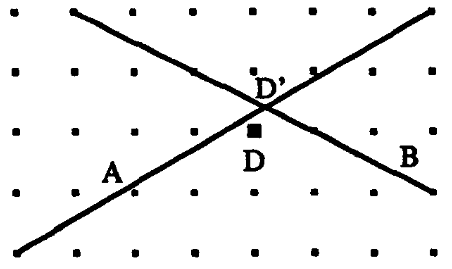
\includegraphics[width=\textwidth]{fig-realms-a.png}
        \caption{}
        \label{fig:realms:redibu:a}
    \end{subfigure}
    \begin{subfigure}[b]{0.3\textwidth}
        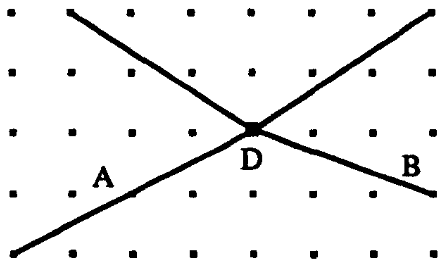
\includegraphics[width=\textwidth]{fig-realms-b.png}
        \caption{}
        \label{fig:realms:redibu:b}
    \end{subfigure}
    \caption{Redibujado de la intersección de dos segmentos.}
    \label{fig:realms:redibu}
\end{figure}

% Envolturas
Pero ahora nos surge un nuevo problema que es la preocupación de que aplicando esta operación sucesivamente
los segmentos se modifiquen cada vez mas, introduciendo cada vez mas error en la representacion.
Podemos acotar este error que se introduce, usando el concepto de envoltura.
La envoltura de un segmento es el conjunto de puntos de la grilla que se encuentran inmediatamente arriba, debajo o sobre el segmento.
Si establecemos entonces la restriccion de que los puntos a usar para el redibujado deben caer sobre la envoltura del segmento,
tenemos una cota para el error: la distancia entre puntos en la grilla.
La figura \ref{fig:realms:envoltura} muestra un ejemplo de envoltura de un segmento.

\begin{figure}
    \centering
    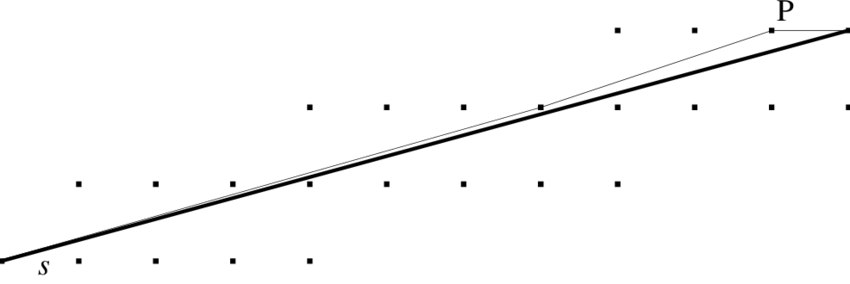
\includegraphics[width=\textwidth]{fig-realms_envoltura.png}
    \caption{Envoltura de un segmento.}
    \label{fig:realms:envoltura}
\end{figure}

% Conclusion
De esta forma, Güting y Schneider definen un conjunto de operaciones geométricas primitivasrobustas con error acotado que son la base para,
a través de la composición de las mismas, definir de forma rigurosa todos los SDTs
y las operaciones geométricas que nos pueden resultar interesantes para la representación de datos espaciales.
Si bien el Álgebra de RoSE fue un hito en términos de rigurosidad teórica en los modelos de bases de datos espaciales,
no es utilizada actualmente en ninguno de los SDBMSs actualmente en uso por la industria del software.
De todas formas, su influencia puede verse en los modelos que se utilizan actualmente y que veremos a continuación.

\subsection{Modelo Funcional}

En esta sección, veremos el modelo funcional o modelo orientado a campos. Comenzaremos presentando un ejemplo de un problema espacial a modelar. Supongamos un parque nacional que cuenta con:
\begin{itemize}
    \item Un conjunto de bosques, cada uno con una especie de árbol dominante.
    \item Un conjutno de instalaciones (oficinas, zonas de campamento, estaciones de bomberos).
    \item Un conjunto de caminos.
    \item Un conjunto de ríos.
    \item Un administrador
\end{itemize}

En el modelo funcional, se pueden modelar los bosques del parque nacional como una función cuyo dominio es es el espacio geográfico subyacente y el rango es un conjunto de especies de árboles. En este caso, la función es una step-function (constante donde en un mismo bosque y con saltos en los bordes entre bosques).

En general, para modelar un problema usando el paradigma funcional, se deben definir tres componentes: un sistema de referencia espacial, funciones de campos y operaciones de campos [Worboys, 1995].

Un sistema de referencia espacial es una grilla finita sobre el espacio subyacente. El ejemplo mas conocido de sistema de referencia espacial es un sistema de referencia de la tierra por latitud y longitud.

Un conjunto finito de n funciones computables o campos simples {fi, 1 <= i <= n},

[funcion]

asigna a cada punto del sistema de referencia F un elemento de un conjunto valores de atributos.

Las relaciones e interacciones entre los diferentes campos se representan con operaciones de campos. Las operaciones de campos mapean un subconjunto de campos en otros campos. La unión + y la composición [TODO: signos de operaciones] son ejemplos de operaciones de campos:

[definiciones]

Las operaciones de campos pueden clasificarse en locales, focales y zonales. Los resultados de las operaciones locales dependen solo de los valores de la entrada en esa ubicación, mientras que las focales dependen también de los valores alrededor de la entrada. Las operaciones zonales trabajan con datos agregados o integraciones.

Los modelos funcionales son buenos para representar problemas en los que las datos continuos como elevación, temperatura y variación del suelo. Tienen la ventaja de poder representar fenómenos espaciales amorfos o con contornos fluidos.

\subsection{Modelos Basados en Objetos}

Volviendo al ejemplo del parque nacional, si consideramos los lugares donde los bosques cambian, en un entorno idealizado donde los bordes entre bosques están claramente definidos, obtendremos un bordes de de polígonos. A cada polígono se le puede asignar una ID y un atributo no espacial (la especie de árbol dominante). Los bosques del parque pueden modelarse entonces como un conjunto de polígonos.

En el modelado basado en objetos, se abstrae información espacial en conjuntos de entidades únicas, distinguibles y relevantes llamadas objetos. Cada objeto tiene un conjunto de atributos que lo caracterizan, los cuales se dividen en atributos espaciales y no espaciales. En el ejemplo del parque nacional, un objeto bosque tiene un atributo espacial, un polígono, que representa su extensión espacial, y un atributo no espacial, su espacie dominante, representada como un valor alfanumérico. Es interesante notar que un objeto puede tener varios atributos espaciales. Por ejemplo, un camino puede tener un polígono y una línea, para elegir cuál usar según la escala del mapa.

Los modelos de objetos son los mas comunes en problemas relacionados a representar redes de transportes o parcelas de tierra. Tienen la ventaja de ser mas intuitivos y cercanos a los modelos Entidad-Relación ya muy presentes en los DBMS más usados. En definitiva, la decisión de usar el paradigma funcional o de en objetos se basará en los requerimientos de la aplicación.

En las próximas secciones, detallaremos más los SDTs y operaciones espaciales en el modelo basado en objetos.

\subsection{SDTs}
Se han propuesto muchos conjuntos básicos de tipos espaciales para la representación de formas comunes en mapas. Actualmente, la más adoptada es el estándar OGIS [OGIS, 1999] y es en la que nos basaremos.
El estándar OGIS propone los siguientes tipos de datos:
\begin{itemize}
    \item Geometría: es un tipo abstracto (no puede ser instanciado) del cual se derivan todos los otros tipos. Tiene asociado un sistema de referencia.
    \item Punto: describe la posicion de objetos de cero dimensiones, como una oficina o una zona de campamento, en el caso del parque nacional.
    \item Cadena de Lineas: describe un objeto de una dimension a través de una sucesión de de dos o mas puntos, que pueden representar un segmento o aproximar una curva. Por ejemplo, caminos o ríos.
    \item Polígono: objetos de 2 dimensiones, como un bosque.
    \item Colección de Geometrías: formas complejas formadas por conjuntos de otros tipos. Se dividen en multipuntos, multilineas y multipoligonos. Estos tipos son necesarios para asegurar que las operaciones geométricas sean cerradas. Por ejemplo, la intersección de un río con un bosque de forma cóncava pueden ser varias líneas.
\end{itemize}

\subsection{Operaciones Espaciales}

En el modelo funcional, las operaciones disponibles quedaban definidas por las funciones de campos del modelo. Pero en un modelo basado en objetos, el espacio subyacente será el que determine las operaciones disponsibles y las relaciones que pueden existir entre objetos. 

\begin{itemize}
    \item Orientado a Conjuntos: son los espacios mas simples y generales. Permiten todas las relaciones usuales de conjuntos como unión, intersección, contención y pertenencia.
    \item Topológicos: los espacios topológicos son aquellos en los que las relaciones no se ven afectadas por transformaciones elásticas del mismo. Relaciones como meet, within y overlap son ejemplos de ejemplos de las disponibles en espacios topológicos.
\end{itemize}

[operaciones dinamicas]

\section{Expandiendo sobre el espacio} \label{sec:e4}
[Generalizacion a N dimensiones]

[El espacio como indice universal]